\documentclass[a4paper,11pt]{article}
\usepackage[utf8]{inputenc}
\usepackage[paper=a4paper, hmargin=1.5cm, bottom=1.5cm, top=3.5cm]{geometry}
\usepackage[T1]{fontenc}
\usepackage[spanish]{babel}
\usepackage[colorlinks=true, linkcolor=blue]{hyperref} %Links para el indice.
\usepackage{amsfonts}
\usepackage{graphicx}
\usepackage{float}
\usepackage{verbatim}
\usepackage{listings}
\usepackage{algorithm}
\usepackage{algpseudocode}
\usepackage{graphicx}
\usepackage{caption}
\usepackage{subcaption}

\usepackage[section]{placeins}
\usepackage{float}
%\usepackage{adjustbox}
\usepackage{amsmath}
\usepackage{blindtext}
\usepackage{sidecap}
\usepackage{color}

% \newcommand{\real}{\hbox{\bf R}}

\title{Trabajo Práctico de Métodos Númericos}
\author{Castro, Dami\'an \& Matayoshi, Leandro \& Szyrej,Alexander}

\begin{document}

\maketitle

\begin{center}
	Universidad de Buenos Aires - Departamento de Computaci\'on - FCEN
\end{center}

%\rule{\linewidth}{1 cm}
\rule{16 cm}{0.5 mm}

\vspace{2cm}

Integrantes:
\begin{itemize}
	\item Castro, Dami\'an L.U.: 326/11  \verb+ltdicai@gmail.com+
	\item Matayoshi, Leandro L.U.: 79/11 \verb+leandro.matayoshi@gmail.com+
	\item Szyrej, Alexander L.U.: 642/11   \verb+alexanderszyrej@gmail.com+
	
\end{itemize}

\vspace{2cm}

\begin{abstract}
  COMPLETAR
\end{abstract}

\vspace{2cm}

Palabras Clave:
\begin{itemize}
	\item PageRank
	\item Extrapolaci\'on Cuadr\'atica
	\item Matriz esparza
\end{itemize}



\newpage

\tableofcontents

\newpage

\section{Introducción teórica}

El algoritmo PageRank se basa en la construcci\'on de un modelo probabil\'istico en base a una red de p\'aginas. Definimos una red de p\'aginas como un conjunto de $n$ p\'aginas y donde hay v\'inculos o links que las unen de forma unidireccional. Esto significa que puedo ir desde la p\'agina $i$ a la p\'agina $j$ si existe un link desde la p\'agina $i$ a la $j$. Dichos links se ven reflejados en lo que llamamos matriz de conectividad $W \in \{0,1\}^{n\times n}$. Diremos entonces que:

\[ w_{ij} =
\begin{cases}
	1 & \text{si existe un link desde la p\'agina $j$ a la $i$ }\\
	0 & \text{si no}
\end{cases}
\]

Adem\'as afirmamos que no existen links de una p\'agina a s\'i misma, de modo que en la diagonal de $W$ hay siempre 0. Con la informaci\'on de esta matriz podemos obtener cuantos links salen desde la p\'agina $i$ viendo la columna $i$ de $W$ y sumando todos los valores. Entonces definimos como grado de p\'agina $n_{k}$  donde:

\[ n_{k} = ||columna_{k}(W)||_{1}\]

Lo importante de este modelo es poder asignarle a cada p\'agina un puntaje, un valor que la distinga de las dem\'as. Diremos que una p\'agina es m\'as importante que otra si tiene un puntaje mayor. Una forma de lograr esto es decir que el puntaje de una p\'agina $i$ es igual a la cantidad de links de llegada a la p\'agina. Esto trae un problema, as\'i que buscamos una manera para que tambi\'en influya la importancia de la p\'agina que posee el link a la p\'agina $i$. Para resolver esto pedimos que, para $k = 1,...,n$:


\[ x_{k} = \sum_{j\in L_{k}}\frac{x_{j}}{n_{j}} \] donde $L_{k}$ es el conjunto de las p\'aginas que tienen un link a la p\'agina $k$. En principio estos valores no son conocidos pero veremos m\'as adelante c\'omo calcularlos.

Entonces definimos $P \in \mathbb{R}^{n\times n}$ de la siguente manera:

\[ p_{ij} =
\begin{cases}
	\frac{1}{n_{j}} & \text{si } w_{ij}\\
	0 & \text{si no}
\end{cases}
\]

Para poder utilizar un an\'alisis probabil\'istico necesitamos que todas las p\'aginas tengan links salientes, a fin de evitar quedarse atascado en una p\'agina. Para lograr esto definimos $v \in \mathbb{R}^{n}$ y $d \in \{0,1\}^{n}$ tal que:

\[ v_{i} = \frac{1}{n} \text{ para } i = 1, \dots, n\]

\[ d_{i} = \\
	\begin{cases}
		1 & \text{si } n_{i} = 0\\
		0 & \text{sino}
	\end{cases}
\]
 
De modo que la nueva matriz que contempla el caso de los links colgantes queda constru\'ida de la siguente manera:

\[ P_{1} = P + vd^{t}\]

Otro fen\'omeno que nos gustar\'ia contemplar es el del \emph{teletransportaci\'on}. Esto implica que desde una p\'agina puede saltarse a cualquier otra p\'agina independientemente de los vecinos de la p\'agina actual. Esto viene asociado con una probabilidad $c \in [0,1]$ tal que el modelo resultante es:

\begin{align*}
	E &= v[1]^{t}\\
	P_{2} &= cP_{1} + (1-c)E
\end{align*}

Se puede observar que $P_{2}$, al igual que $P_{1}$ es estoc\'astica por columnas y por lo tanto cumple las hip\'otesis planteadas en Bryan y Leise\cite{Bryan2006} y Kamvar et al.\cite{Kamvar2003} , y por esta raz\'on $P_{2}$ tiene un autovector asociado a un autovalor $\lambda_{1} = 1$ y tal que $\lambda_{1} > |\lambda_{2}| > \dots |\lambda_{n}|$. De esta manera se puede utilizar el sistema $P_{2}x = x$ para hallar dicho autovector.


Veremos entonces que podemos utilizar el m\'etodo de la potencia para hallar ese autovector ya que dicho autovector est\'a asociado al autovalor m\'aximo de $P_{2}$. Luego, por la secci\'on 5.2 se puede observar que realizar el c\'alculo para m\'etodo de la potencia es equivalente a realizar el procedimiento ah\'i explicado. Realizar el c\'alculo de esa forma es conveniente ya que aprovecha que la matriz $P_{2}$ proviene de una matriz esparsa $P$.

\section{Desarrollo}

\subsection{Implementaci\'on de matriz esparsa.}


Dado el inmenso tama\~no de la Web en general y considerando que el algoritmo de PageRank puede darse para un subconjunto muy grande de esta Web es necesario contemplar los requisitos de espacio f\'isico intr\'insecos a nuestro problema. As\i mismo, visto que trabajamos con matrices esparsas, fue necesario crear un m\'odulo que tome ventaja de esta propiedad, y que de esta manera minimice el espacio requerido.


%yale format init
Una primera aproximaci\'on fue basarnos en el formato Yale para matrices esparsas, el cual cuenta con tres arreglos:
\begin{itemize}
	\item A : valores distintos de cero pertenecientes a la matriz.
	\item IA : indices en A para los primeros valores de cada fila.
	\item JA : n\'umero de columna para cada valor de A.
\end{itemize}

Este formato parec\'ia ahorrar una cantidad considerable de espacio en memoria, pero surg\'ian problemas a medida que aparec\'ian filas que no conten\'ian ning\'un valor distinto de cero, algo que puede suceder tranquilamente. De repente el arreglo IA se volv�a inconsistente y dejaba de tener sentido.
%yale format out


Finalmente decidimos implementar SparseMatrix en base a un vector de listas, donde cada lista representa una fila (puede ser vacia) y cuyos elementos, de existir, son pares <valor,columna>. No s\'olo simplific\'o la implementaci\'on evitando as\'i mismo el absurdo almacenamiento de los valores nulos, sino que tambi\'en mejora el tiempo de ejecuci\'on para la multiplicaci\'on Matriz-Vector, dado que �nicamente se toman en consideraci�n los valores no nulos de cada fila y cada uno viene acompa�ado del \'indice del valor en el vector con el cual de lo debe multiplicar.

\subsection{M\'etodo de la potencia optimizado}

El m\'etodo de la potencia \cite[Secci\'on 9.3]{Burden} es un algoritmo que me permite hallar el m\'aximo autovalor de una matriz, junto a su autovector. La idea principal del m\'etodo es multiplicar un vector sucesivas veces por una matriz. El resultado de realizar esto es que el vector original se transforma seg\'un los autovalores de la matriz y se orienta seg\'un los autovectores de la misma. Si existe un autovalor que es dominante, o sea, es m\'as grande que el resto de los dem\'as, es intuitivo pensar que el vector que es multiplicado se transforme seg\'un ese autovalor y apunte a la direcci\'on de dicho autovector. Ahora, como sabemos que el autovalor dominante de la matriz $P_{2}$ es 1 sabemos que el vector no se va a transformar y lo \'unico que va a suceder es que se va a orientar hacia el autovector asociado al autovalor 1, justamente lo que queremos hallar. Sin embargo, cada iteraci\'on del m\'etodo de la potencia involucra una multiplicaci\'on de matriz con vector y es una operaci\'on costosa en tiempo de procesamiento. Ser\'ia conveniente hallar una forma de reducir ese costo.

Seg\'un Kamvar et al. \cite[Algoritmo 1]{Kamvar2003} para hacer el m\'etodo de la potencia para el sistema $P_{2}x = y$ es equivalente a realizar el siguiente m\'etodo.

\vspace{0.5cm}

\begin{algorithmic}
	\Function{Algoritmo 1}{\textbf{vector} $x$}{ $= y$}
		\State $a = cPx$
		\State $b = ||x||_{1} - ||a||_{1}$
		\State $y = a + bv$
		\State \Return $y$
	\EndFunction
\end{algorithmic}

\vspace{0.5cm}

De modo que el m\'etodo de la potencia queda estructurado de la siguiente manera.

\vspace{0.5cm}

\begin{algorithmic}
	\Function{power method}{}{ $= x^{(n)}$}
		\State \textbf{vector} $x^{(0)} \gets v$
		\State $k \gets 1$ \Repeat
		\State $x^{(k)} \gets \text{Algoritmo 1}(x^{(k-1)})$
		\State $\delta \gets ||x^{(k)} - x^{(k-1)}||_{1}$ \Until $\delta < \epsilon$
		\State \Return $x^{(k)}$
	\EndFunction
\end{algorithmic}

\vspace{0.5cm}

El m\'etodo itera varias veces hasta que la diferencia entre dos iteraciones sucesivas sea menor a un $\epsilon$ dado. Como podemos asegurar convergencia a partir de cualquier $x^{(0)}$ ya que la matriz $P_{2}$ es estoc\'astica por columnas por lo tanto se cumple la proposici\'on 5  exhibida en Bryan \& Leise \cite[Secci\'on 4]{Bryan2006}.

Sin embargo, cada iteraci\'on del m\'etodo de la potencia lleva bastante tiempo, incluso con el Algoritmo 1, as\'i que es necesario tratar de acelerar la convergencia de alguna manera. Esto lo lograremos con el siguiente algoritmo, extrapolaci\'on cuadr\'atica.


\subsection{Extrapolaci\'on cuadr\'atica}

El m\'etodo de extrapolaci\'on cuadr\'atica \cite[Secci\'on 4]{Kamvar2003}consiste en asumir que la matriz $P_{2}$ tiene solo 3 autovectores con 3 autovalores asociados y por lo tanto $x^{(k-3)}$ se puede escribir como combinaci\'on lineal de esos autovectores. Esto nos va a permitir entonces hallar una f\'ormula cerrada para calcular $x^{(k+1)}$ en base a las iteraciones anteriores $x^{(k-3)} \dots x^{(k)}$. Por supuesto, la matriz $P_{2}$ tiene m\'as autovectores que 3 y por lo tanto el valor obtenido es una aproximaci\'on al valor real. Sin embargo, se observa que, a medida que aumenta la cantidad de iteraciones esa aproximaci\'on es bastante buena.

Si suponemos que la matriz tiene solo 3 autovectores $x^{(k-3)}$ se puede escribir como combinaci\'on lineal de esos autovectores:

\[
	x^{(k-3)} = u_{1} + \alpha_{2}u_{2} + \alpha_{3}u_{3}
\]

Luego podemos escribir a las iteraciones sucesivas de la siguiente manera:

\begin{align*}
	x^{(k-2)} &= P_{2}x^{(k-3)}\\
	x^{(k-1)} &= P_{2}x^{(k-2)}\\
	x^{(k)} &= P_{2}x^{(k-1)}
\end{align*}

Luego sea $p$ el polinomio car\'acteristico de $P_{2}$ es un polinomio de grado 3. Las ra\'ices del polinomio son los autovalores de la matriz, en especial el autovalor que conocemos, 1. Evaluando el polinomio en 1 obtenemos:

\[
	p(1) = \gamma_{0} + \gamma_{1} + \gamma_{2} + \gamma_{3} = 0
\]

Luego definamos lo siguiente:

\begin{align*}
	y^{(k-2)} =& x^{(k-2)}- x^{(k-3)} \\
	y^{(k-1)} =& x^{(k-1)}- x^{(k-2)}\\
	y^{(k)} =& x^{(k)}- x^{(k-1)}
\end{align*}

En Kamvar et al.[Secci\'on 5]\cite{Kamvar2003} se utiliza un teorema que me dice que evaluar el polinomio car\'acter\'istico en la matriz $P_{2}$ y multiplicarlo por cualquier vector $z \in \mathbb{R}^{n}$ y el resultado es igual a 0. Adem\'as, sea $z = x^{(k-3)}$, entonces resulta que:

\begin{align*}
	p(P_{2})x^{(k-3)}	=& [\gamma_{0}I + \gamma_{1}P_{2} + \gamma_{2}(P_{2})^{2} + \gamma_{3}(P_{2})^{3}]x^{(k-3)} = 0 \\
						=& \gamma_{0}x^{(k-3)} + \gamma_{1}x^{(k-2)} + \gamma_{2}x^{(k-1)} + \gamma_{3}x^{(k)}= 0 \\
						=& (- \gamma_{1} - \gamma_{2} - \gamma_{3})x^{(k-3)} + \gamma_{1}x^{(k-2)} + \gamma_{2}x^{(k-1)} + \gamma_{3}x^{(k)}= 0 \\
						=& (x^{(k-2)}- x^{(k-3)})\gamma_{1} + (x^{(k-1)}- x^{(k-3)})\gamma_{2} + (x^{(k)}- x^{(k-3)})\gamma_{3}\\
						=& y^{(k-2)}\gamma_{1} + y^{(k-1)}\gamma_{2} + y^{(k)}\gamma_{3}
\end{align*}

Esto se puede escribir en forma matricial de esta manera:

\begin{align}
	\left(y^{(k-2)} \quad  y^{(k-1)} \quad  y^{(k)}\right)\gamma = 0 \label{sistmat}
\end{align}

Como no estamos interesados en la soluci\'on trivial $\gamma = 0$, pediremos que $\gamma_{3} = 1$. Por lo tanto el sistema \eqref{sistmat} puede reescribirse como:

\begin{align}
	\left(y^{(k-2)} \quad y^{(k-1)}\right)\gamma = - y^{(k)} \label{sistmat2}
\end{align}

Resolviendo ese sistema hallamos los valores de $\gamma$(veremos m\'as adelante como realizaremos este paso) y por lo tanto los coeficientes del polinomio $p$. Ahora, sea $q$ un polinomio definido de la siguiente manera:

\begin{align}
	q(\lambda) = \frac{p(\lambda)}{(1-\lambda)} = \beta_{0} + \beta_{1}\lambda + \beta_{2}\lambda^{2} \label{polq}
\end{align}

Como ya sabemos los valores de $\gamma$ podemos despejar los valores de $\beta_{i}$ de manera que:

\begin{align*}
	\beta_{0} &= \gamma_{1} + \gamma_{2} + \gamma_{3} \\
	\beta_{1} &= \gamma_{2} + \gamma_{3} \\
	\beta_{2} &= \gamma_{3}
\end{align*}

Nuevamente por el teorema utilizado anteriormente vale que para cualquier vector $r$:

\[
	q(P_{2})r = u_{1}
\]

Sea $r = x^{(k-2)}$ entonces vale la siguiente igualdad

\begin{align*}
	q(P_{2})x^{(k-2)} =& [\beta_{0}I + \beta_{1}P_{2} + \beta_{2}(P_{2})^{2}]x^{(k-2)}\\
	u_{1} =& \beta_{0}x^{(k-2)} + \beta_{1}x^{(k-1)} + \beta_{2}x^{(k)}
\end{align*}

Y eso es justamente lo que quer\'iamos obtener. Por lo tanto tenemos una nueva aproximaci\'on a $u_{1}$ basado en valores anteriores de la sucesi\'on $\{x^{(n)}\}$.

Nos queda por decidir como resolver el sistema planteado en \eqref{sistmat2} de forma eficiente de manera que realizar extrapolaci\'on quadr\'atica no sea costosa. Definimos lo siguiente:

\[
	Y = \left(y^{(k-2)} \quad y^{(k-1)}\right)
\]


Se observa que $Y$ es un sistema sobredeterminado ya que hay m\'as filas que columnas, por lo tanto la soluci\'on obtenida es aquella de resolver el problema de cuadrados m\'inimos. Una forma de encontrar la soluci\'on de cuadrados m\'inimos es utilizando la factorizaci\'on QR. Dicha factorizaci\'on consiste en poder descomponer la matriz $Y \in \mathbb{R}^{n \times 2}$ en el producto de dos matrices: $Q\in \mathbb{R}^{n \times n}$ y $R\in \mathbb{R}^{n \times 2}$, de manera que:

\begin{align*}
	Y\gamma &=-y^{(k)}\\
	QR\gamma &=-y^{(k)}\\
	R\gamma &=-Q^{t}y^{(k)}\\
\end{align*}

\begin{figure}[!h]
	\begin{center}
		  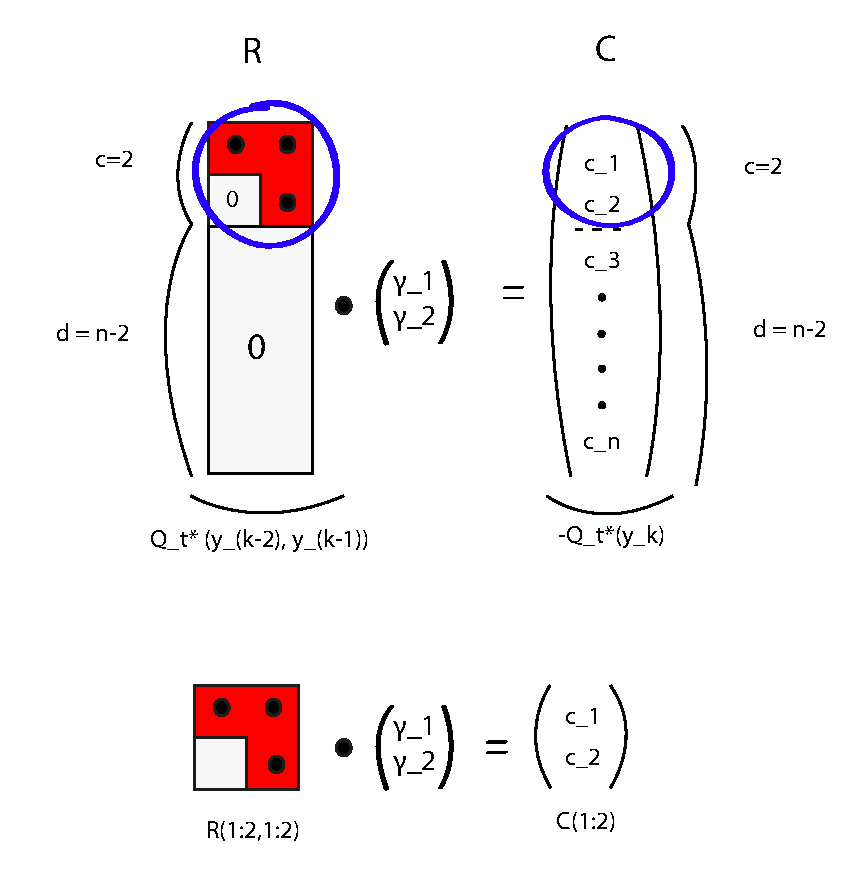
\includegraphics[scale = 0.5]{graficos/im_1.pdf}
		  \caption{Sistema a resolver simplificado}
		  \label{fig:contra1}
	\end{center}
\end{figure}
\FloatBarrier
Y esto resulta un sistema f\'acil para resolver utilizando \emph{backwards-substitution}.

Uno de los m\'etodos vistos en la materia para obtener la factorizaci\'on QR fue el m\'etodo de \emph{Householder} \cite{Burden} que me permite reflejar ortogonalmente las columnas de $Y$ y as\'i ir obteniendo la matriz triangular superior $R$. Se puede observar que como la matriz $Y$ tiene solo 2 columnas entonces en 2 pasos de \emph{Householder} se obtiene la $R$ deseada. El problema es la dimensi\'on de $Q$. Al ser $n$ muy grande (que es lo esperado), calcularla en base al producto de $Q_1$ (primer paso de \emph{Householder}) y $Q_2$ (segundo paso de \emph{Householder}) es muy costoso en cuanto a recursos de memoria. Con \emph{web-Stanford} como entrada, la factorizaci\'on $QR$ cuelga el sistema ya que se queda sin memoria. 

Es por esto que implementamos \emph{Householder eficiente}, donde buscamos obtener $R$ y $-Q^{t}y^{(k)}$ a trav\'es de sucesivas multiplicaciones del tipo Matriz-Vector, y resta de matrices. Evitar el almacenamiento en memoria y producto de matrices de $n \times n$ es importantisimo en el contexto de este trabajo, ya que hablamos de un \'orden de $O(n^3)$ para el producto y $O(2*n^2)$ en memoria.

A continuaci\'on, el primer paso de \emph{Householder eficiente}. El segundo es an\'alogo.

~

$(I - 2uu^{t})*A = (I - 2uu^{t})*b$

$(A - 2uu^{t}A) = (b - 2uu^{t}b)$

~

Notemos que $u^{t}*b$ es un escalar (por lo que simplifica mucho las operaciones). Además no tenemos que multiplicar por la 
identidad ya que el paso resulta trivial.

Volviendo al problema de hallar $P_{2}x = y$, el algoritmo con la optimización es entonces: 

~

\begin{algorithmic}
	\Function{power method with quadratic extrapolation}{}{ $= x^{(n)}$}
		\State \textbf{vector} $x^{(0)} \gets v$
		\State $k \gets 1$ \Repeat
		\State $x_{k-3} \gets x_{k-2}$
		\State $x_{k-2} \gets x_{k-1}$
		\State $x_{k-1} \gets x_{k}$
		\State $x^{(k)} \gets \text{Algoritmo 1}(x^{(k-1)})$
		\If{someConditionAboutk}
			\State $x^{(k)} \gets$ QuadraticExtrapolation($x_{k-3},x_{k-2},x_{k-1},x_{k}$)
		\EndIf
		\State $\delta \gets ||x^{(k)} - x^{(k-1)}||_{1}$ \Until $\delta < \epsilon$
		\State \Return $x^{(k)}$
	\EndFunction
\end{algorithmic}





\section{Resultados y discusión}



\subsection{Experimento 2: Variando la periodicidad de Extrapolaci\'on cuadr\'atica}

Si bien el m\'etodo de extrapolaci\'on cuadr\'atica ayuda a la convergencia general del m\'etodo de la potencia, su costo es mucho mayor al ciclo principal del m\'etodo mencionado. Es por esto que, para realmente acelerar el ritmo de convergencia es necesario realizar la extrapolaci\'on cuadr\'atica de manera peri\'odica y no en cada iteraci\'on.

Pero, ¿Cual es la distancia \'optima entre iteraciones en las que debemos realizar la extrapolaci\'on? ¿Disminuyen las iteraciones totales si se aplica la extrapolaci\'on cuadr\'atica de manera cercana? ¿Y qu\'e sucede con el tiempo?

Para responder a todas estas preguntas, planteamos dos pequeños experimentos en base al grafo $web-Stanford$ de aproximadamente 280mil nodos:

\begin{itemize}
	\item Analizar la relaci\'on periodicidad-\#IteracionesTotales variando la distancia entre iteraciones en las que usamos la Extrapolaci\'on Cuadr\'atica.
	\item Analizar la relaci\'on periodicidad-tiempo operando de la misma forma que en el item anterior pero realizando varias repeticiones de cada experimento para promediar los tiempos y evitar valores incoherentes propios del scheduling de nuestro sistema operativo.
\end{itemize}

~

Los resultados fueron los siguientes:

\begin{center}
    \small{
    \begin{tabular}{| l | l |}
    \hline
    Distancia entre iteraciones con extrapolaci\'on & \#Iteraciones\_Totales \\ \hline
    5 & 75 \\ \hline
    7 & 71 \\ \hline
    10 & 71 \\ \hline
    20 & 73 \\ \hline
    30 & 72 \\ \hline
    40 & 74 \\ \hline
    50 & 74 \\ \hline

    \end{tabular}
    }
\end{center}
\begin{center}
c = 0.80. Epsilon = $10^{-10}$.
\end{center}

~

Si bien la cantidad de iteraciones totales disminuye con extrapolac\'ion cuadr\'atica respecto del m\'etodo cl\'asico de la potencia, puede apreciarse en la tabla que su periodicidad en la aplicaci\'on no modifica en gran medida la cantidad total de iteraciones para el mismo m\'etodo, contrario a lo que cre\'iamos inicialmente. 

Sin embargo, fue notorio durante el trayecto de este experimento que los tiempos iban cambiando a medida que se produc\'ian menos llamadas a extrapolaci\'on cuadr\'atica, lo cual era de esperarse debido al costo dicho m\'etodo.

Seg\'un estos resultados, creemos que realizar extrapolaci\'on cada 10 iteraciones es un buen criterio para minimizar la cantidad de ciclos en base a un grafo de entrada de caracter\'isticas similiares.

~

A continuaci\'on, los resultados obtenidos respecto del tiempo total de ejecuci\'on. 


\begin{center}
    \small{
    \begin{tabular}{| l | l |}
    \hline
    Distancia entre iteraciones con extrapolaci\'on & Tiempo (en millones de ciclos) \\ \hline
    7 & \textcolor{red}{\~21} \\ \hline
    10 & 16.4
    15 & 12.06 \\ \hline
    25 & 9 \\ \hline
    35 & 8.85 \\ \hline
    45 & 7.48 \\ \hline
    
    \end{tabular}
    }
\end{center}
\begin{center}
c = 0.80. Epsilon = $10^{-10}$. Tiempos medidos en base a $tiempo.h$ otorgado por la c\'atedra de Orga2.
\end{center}

Dado que el algoritmo de power-method-with-quadratic-extrapolation es costoso en terminos de tiempo con grafos de entrada suficientemente grandes, se realizaron s\'olo 5 repeticiones de las mediciones para acortar tiempos. 

Podemos apreciar el gran costo de aplicar el m\'etodo de extrapolaci\'on cuadr\'atica de forma $demasiado$ peri\'odica viendo el tiempo total que tarda el algoritmo si las iteraciones de extrapolaci\'on son muy cercanas.

Observando la tabla podemos ver que el tiempo disminuye a medida que se aplica el m\'etodo de manera mas distanciada, acelerando la convergencia de manera periodica sin retrasar el tiempo total con sucesivas llamadas al costoso proceso de extrapolaci\'on cuadr\'atica.









\input{tiempos.tex}

\section{Conclusiones}

Durante el transcurso de este trabajo fuimos analizando el m\'etodo de la potencia en contraposici\'on con la mejora de extrapolaci\'on cuadr\'atica. Los resultados obtenidos no siempre fueron los esperados, pero en lineas generales entendemos que la extrapolaci\'on cuadr\'atica es realmente una mejora al momento de hallar el autovector asociado al m\'aximo autovalor $\lambda = 1$ de una matriz con la propiedad de ser una cadena de Markov, siempre y cuando se lo aplique de manera peri\'odica no demasiado consecutiva.

Al trabajar con grafos de mayor tama\~no en cuanto a cantidad de nodos, ambos m\'etodos se comportan como es de esperarse. Siempre el m\'etodo que implementa la extrapolaci\'on cuadr\'atica converge m\'as rapido que el m\'etodo cl\'asico de la potencia en cuanto a cantidad de iteraciones. Igualmente a medida que la entrada aumenta en tama\~no se vuelve cada vez mas necesario contar con un m\'odulo que implemente matriz esparsa, y es importantisimo contar con un m\'etodo eficiente para el c\'alculo de la factorizaci\'on $QR$ frente a entradas de gran tama\~no como, por ejemplo, es el caso de $web-Stanford$.

Sin embargo, en cuanto a tiempos, si la extrapolaci\'on se produce de forma muy consecutiva puede provocar un overhead temporal que ralentizar\'ia el tiempo de ejecuci\'on total. Lo mismo no sucede en terminos de convergencia en cuanto a cantidad de iteraciones. Variar la periodicidad de la extrapolaci\'on no influye en la cantidad total de iteraciones. Consideramos que una distancia de entre 10 y 20 iteraciones de por medio entre llamadas al $extrapolation\_method$ es \'optima para un mejor resultado temporal.

En cuanto al valor de $c$, creemos que fijarlo en un valor muy cercano al 1 es deseable para un correcto modelaje del navegador random. Con un valor de 0.80 / 0.85 creemos que sin perder peso en la matriz original podemos incluir el concepto de teletransportaci\'on y es por eso que fijamos en ese valor dicha variable.

%saludos y gracias.


\section{Apéndices}

\subsection{Enunciado}

El objetivo del trabajo es implementar el algoritmo PageRank, considerando dos m\'etodos distintos para el c\'alculo del
autovector principal de la matriz $P_2$. Para ello, se considera el entorno de aplicaci\'on real del algoritmo, donde el
n\'umero total de p\'aginas, $n$, es considerablemente grande (i.e., todas las p\'aginas web accesibles p\'ublicamente).
El programa tomar\'a como entrada un archivo con la representaci\'on de grafo de conectividad, construir\'a la matriz
$P_2$ definida en la secci\'on anterior y ejecutar\'a el algoritmo PageRank utilizando el m\'etodo de la potencia y una 
variante del mismo para distintas instancias de prueba. Se pide:

\begin{enumerate}
\item En base a su definici\'on, $P_2$ no es una matriz esparsa. Sin embargo, en Kamvar et al. \cite[Algoritmo
1]{Kamvar2003} se propone una forma alternativa para computar $x^{(k+1)} = P_2 x^{(k)}$. Mostrar que el c\'omputo
propuesto es equivalente. Utilizarlo para mejorar el espacio requerido en memoria para el almacenamiento de la matriz
$P_2$ y el tiempo de ejecuci\'on requerido para hacer la multiplicaci\'on entre matrices y vectores. 

\item Bas\'andose en el an\'alisis del punto anterior, implementar el m\'etodo de la potencia para calcular el
autovector principal de la matriz $P_2$.

\item Implementar la variante del M\'etodo de la Potencia propuesta en Kamvar et al. \cite[Secci\'on 5]{Kamvar2003},
denominada Extrapolaci\'on Cuadr\'atica. El m\'etodo de Cuadrados M\'inimos involucrado debe ser resuelto utilizando la
Factorizaci\'on QR de la matriz mediante alguno de los m\'etodos vistos en la materia.

\item Realizar experimentos considerando distintas instancias de prueba. Para ello, se podr\'a utilizar el c\'odigo
adjuntada para la generaci\'on de instancias en base a datos reales, o cualquier otra herramienta que el grupo considere
necesaria. Evaluar tambi\'en los algoritmos alguno de los conjuntos de instancias
provistos en \cite{SNAP}. Para cada algoritmo, analizar el tiempo de
ejecuci\'on, la evoluci\'on del error entre iteraciones consecutivas y considerar distintos criterios de parada. 
Adem\'as, analizar la calidad del ordenamiento obtenido en t\'erminos de la relevancia de las p\'aginas.
\end{enumerate}

\subsection{Correctitud del Algoritmo 1 de Kamvar} 
Seg\'un Kamvar et al. se puede reducir el problema de $(P_{2})x = y$ a realizar el siguiente c\'alculo:

	$a = cPx$

	$b = ||x||_{1} - ||a||_{1}$

	$y = a + bv$

Veamos que eso es correcto desarrollando $(P_{2})x$.

\begin{align}
	& P_{2}x = [cP_{1} + (1-c)E]x = [c(P + D) + (1-c)E]x = cPx + cDx + Ex -cEx \nonumber\\
	& \implies cPx + cDx + Ex -cEx = y= cPx +bv \label{ap1}
\end{align}

Se puede observar en \ref{ap1} que ya logramos que se cumpla el primer t\'ermino. Veamos ahora que  

\begin{align*}
	cDx + Ex -cEx &= bv \\
	cvd^{t}x + v[1]^{t}x - cv[1]^{t}x &= bv
\end{align*}

Como $d^{t}x$ y $[1]^{t}x$ son escalares, puedo moverlos a la izquierda del producto

\begin{align}
	(cd^{t}x)v + ([1]^{t}x)v - (c[1]^{t}x)v &= bv \nonumber\\
	(cd^{t}x +[1]^{t}x - c[1]^{t}x)v &= bv \label{ap2}
\end{align}

Entonces, por \eqref{ap2} quiero ver que:
\begin{align}
	(cd^{t}x +[1]^{t}x - c[1]^{t}x) = b = ||x||_{1} - ||a||_{1}\label{ap3}
\end{align}
Se puede observar que como x es un vector de probabilidades entonces todas sus coordenadas son no negativas, y por lo tanto $[1]^{t}x = ||x||_{1}.$

Reemplazo esto en la ecuaci\'on \eqref{ap3}

\begin{align}
(cd^{t}x +[1]^{t}x - c[1]^{t}x) &= [1]^{t}x - ||cPx||_{1} \nonumber\\
(cd^{t}x-c[1]^{t}x) &= -||cPx||_{1} \nonumber\\
-c([1]^{t}x-d^{t}x) &= -c||Px||_{1} \nonumber\\
([1]^{t} -d^{t})x &= ||Px||_{1} = \left(\sum_{i=i}^{n}[fila_{i}(P)]x\right) = \left(\sum_{i=i}^{n}(fila_{i}(P))\right)x \label{ap4}
\end{align}

Entonces bastar\'ia con ver que, $\forall$ $ 1 \leq j \leq n$:

\begin{align}
	([1]^{t} -d^{t})_{j} = \left(\sum_{i=i}^{n}(fila_{i}(P))\right)_{j} \label{ap5}
\end{align}

Analicemos \eqref{ap5} por separado.

Primer lado de la ecuaci\'on. Siendo $d_{out}(k)$ el n\'umero de vecinos de la p\'agina $k$.
\[
	([1]^{t} -d^{t})_{j} = 
	1 - d_{j} = 
	\begin{cases}
		1 & \text{si }d_{j} = 0 \iff d_{out}(j) \neq 0 \\
		0 & \text{si no}
	\end{cases}
\]

Segundo lado de la ecuaci\'on. Como la matriz $P$ tiene todos sus elementos no negativos entonces vale:

\[
	\left(\sum_{i=i}^{n}(fila_{i}(P))\right)_{j} = ||columna_{j}(P)||_{1} =
		\begin{cases}
		1 & \text{si la p\'agina $i$ tiene links salientes } \iff d_{out}(j) \neq 0 \\
		0 & \text{si no}
	\end{cases}
\]

Esto se debe a que la matriz $P$, cuando la columna tiene elementos distintos de 0 entonces cumple que la suma de los elementos de la columna es igual a 1.

Por lo tanto, para mismos valores de $j$ ambos lados de la ecuaci\'on valen lo mismo, entonces puedo asegurar que son iguales. Y con esto demuestro que utilizar el Algoritmo 1 de Kamvar\cite{Kamvar2003} es equivalente a resolver $P_{2}x = y$

\section{Referencias}

\input{referencias.tex}

\section{Código}

\tiny{
\lstset{caption=Codigo de los principales algoritmos: power method con y sin la optimización
, framexleftmargin=2mm, frame=shadowbox, rulesepcolor=\color{black}, language={[ANSI]C}}

\lstinputlisting[language=C++]{codigo/PageRank.cpp}
}




\bibliographystyle{plain}
\bibliography{tp3}

\end{document}
